



\section{Method}
\label{sec:method}
\subsection{Overview}
In this section, we present our precomputed Gaussian splats radiance transfer framework, shown in Fig \ref{pipeline}, which decomposes geometry, materials, and illumination
for Gaussian splats (sec \ref{4.2} and \ref{4.3}). In addition, we developed unique precomputing and ray tracing methods that are specifically tailored to accommodate the unique geometry and rendering pipeline of 3DGS (sec \ref{4.4}). Finally, we recursively compute self-transfer and project radiance transfer into SH coefficients for fast rendering (sec \ref{4.5}).


%如图，稀疏的脉冲流不适合直接作为监督信号。因此，我们使用脉冲发放频率作为低光脉冲流与正常光脉冲流的桥梁。我们提出了首个基于有监督学习的脉冲流增强框架，xxx in fig。具体地，我们先估计xxx(xxx)脉冲流的脉冲发放频率.然后，通过我们的网络学习从低光脉冲流中的脉冲发放频率到正常光脉冲流中的脉冲发放频率。最终，增强脉冲频率序列被解码为增强脉冲流。


% 为了简便，我们写脉冲流为，
%$\mathbb{S}_t = \{ {  S}_{t + i} \in \{0, 1\}^{W \times H} | i = 0, \pm 1,  \pm 2, \dots\}$
%, 其中t是中心时刻而$|\mathbb{S}_t|$是时间窗口。脉冲发放频率序列为

%\subsection{Spike Camera Model with Realistic Noise}


\subsection{BRDF Rendering} \label{4.2}
%如图，我们提出了一个多分支频率增强网络。
To facilitate the physically based rendering of 3D Gaussian splats, we introduce a parametrization scheme that includes an additional set of terms for optimization purposes, \emph{i}.\emph{e}. albedo $\rho \in [0,1]$, roughness $\emph{r} \in [0,1]$ and metallic $\emph{m} \in [0,1]$. According to Disney BRDF model \cite{burley2012physically}, the BRDF property $f(\omega_i,\omega_o)$ of a material can be decomposed into two components: roughness BRDF $f_d$ and specular BRDF $f_s$.
\begin{align}
    f(\omega_i,\omega_o)=(1-\emph{m})\frac{\rho}{\pi}+\frac{DFG}{4(\omega_i \cdot n)(\omega_o \cdot n)}=f_d+f_s
\end{align}
where $D$ is the microfacet distribution function, $F$ is the Fresnel reflection and $G$ is the geometric shadowing factor all of which are related to the roughness \emph{r}.
Then equation \ref{rendering equation} can be written as:
\begin{align}
    L_o(\omega_o)=L_o^s(\omega_o)+L_o^d
\end{align}
where:
\begin{align}
    L_o^d=f_d\int_{\Omega}L_i(\omega_i,x)(\omega_i,n)d\omega_i
\end{align}
\begin{align}
    L_o^s(\omega_o)=\int_{\Omega}f_s(x,\omega_i,\omega_o)L_i(\omega_i,x)(\omega_i,n)d\omega_i
\end{align}
\subsection{Lighting and Geometry Modeling}\label{4.3}
\textbf{Lighting Modeling} The majority of existing methods decompose the incident light $L_i$ at point x into two components: direct illumination $L_i^{dir}$ and indirect illumination $L_i^{in}$. Equation \ref{rendering transfer equation} can be further written as:
\begin{align}
    L_o(\omega_o)=\int_{\Omega}T(\omega_i,\omega_o)(L_i^{dir}(\omega_i)+(L_i^{in}(\omega_i))d\omega_i
\end{align}
However, computing accurate indirect illumination in real-time for 3D Gaussian splats is a challenging task. We precompute self-transfer instead of directly computing indirect illumination. Considering:
\begin{align}
    L_i^{in}(-\omega_i)=\int_{\Omega}T^{1}(\omega_i^{1},-\omega_i)(L_i^{dir}(\omega_i^{1})+(L_i^{in}(\omega_i^{1}))d\omega_i^{1}
\end{align}
where $T^{1}(\omega_i^{1},-\omega_i)$ is the light transfer at point (splat) $x^1$ which is hit by one-bounce ray tracing.
Recursively, we have:
\begin{align}
    L_o(\omega_o)=\int_{\Omega}T'(\omega_i,\omega_o)L_i^{dir}(\omega_i)d\omega_i \label{recu}
\end{align}
where 
% \begin{align}
% T'(\omega_i,\omega_o)=T(\omega_i,\omega_o)+\int_{\Omega}T^1(\omega_i^1,-\omega_i)+\dots+\int_{\Omega}\dots\int_{\Omega}T^n(\omega_i^n,-\omega_i^{n-1})d\omega^n
% \end{align}
\begin{align}
\label{recu2}
&T'(\omega_i,\omega_o)=T(\omega_i,\omega_o)+T(\omega_i,\omega_o)\int_{\Omega}T^1(\omega_i^1,-\omega_i)d\omega^1_i\\
&+\dots+T(\omega_i,\omega_o)\int_{\Omega}\dots \int_{\Omega}T^n(\omega_i^n,-\omega_i^{n-1})d\omega^n_i \nonumber
\end{align}
and
the global direct light term $L_{dir}$ is parameterized as a globally shared SH, denoted as $\Vec{l_{dir}}$, and indirect light is represented as the direct light multiplied by self-transfer.

\hupar{Geometry Modeling} Same as \cite{gao2023relightable,liang2023gsir,jin2023tensoir,zhang2021nerfactor}, we utilize the depth gradient to derive pseudo-normals, which in turn serve as guidance for optimizing normals within the 3D Gaussian splats. Given the distance from the corresponding 3D Gaussian splat to the image plane $d_i$ and the $\alpha_{i}$ by evaluating a 2D Gaussian with covariance $\Sigma$ multiplied with a learned per-point opacity, we obtain pseudo depth D derived from equation \ref{point rendering}:
\begin{align}
    D=\sum_{\substack{i\in N}}d_{i}\alpha_{i}\prod_{j=1}^{i-1}(1-\alpha_{j})
\end{align}
The pseudo-normal $N' \in HxW$ can be computed from D. 
However, calculating the normal $n_i$ for each Gaussian from 
$N$ through interpolation is highly inaccurate. Therefore, like \cite{gao2023relightable,jin2023tensoir}, we initialize a random normal $n_i$ for each Gaussian splat and constrain it using normal loss $L_{normal}$. Here:
\begin{align}
    L_{normal}=\|N-N'\| 
\end{align}
and
\begin{align}
    N=\sum_{\substack{i\in N}}n_{i}\alpha_{i}\prod_{j=1}^{i-1}(1-\alpha_{j})
\end{align}
\subsection{3D Gaussian Raytracing}\label{4.4}


 In the context of 3D Gaussian splats, the computational overhead of ray tracing is notably increased. Because ray tracing cannot be initiated directly from screen space, multiple sampling is required for each Gaussian splat to achieve noise-free results. Moreover, rays need to bounce recursively between Gaussian splats, as the number of bounces increases, the computation for tracing and rendering grows exponentially with the sample amount. In this paper, we present a novel ray tracing technique integrated with self-transfer precomputation. Our approach streamlines the process by doing one-bounce ray tracing during the whole training or rendering stage and updating self-radiance transfer iteratively and recursively. As a result, we achieve precise computation of indirect illumination for multiple bounces under diverse dynamic environment lighting. Like \cite{gao2023relightable,liang2023gsir,chen2023gaussianeditor}, our proposed ray tracing technique on 3D Gaussian splats is constructed upon the Bounding Volume Hierarchy (BVH), facilitating efficient querying of visibility along a ray. 
Unlike conventional ray tracing methods, our approach does not involve computing irradiance during the ray tracing process. Instead, we solely compute the weights $W_i$ of the Gaussian splat intersected along each direction and record the index of the Gaussian splat with the maximum weight for each direction. Same as \ref{point rendering}, our weight can be written as:
\begin{align}
    W_i=\alpha_{i}\prod_{j=1}^{i-1}(1-\alpha_{j})max(-r_d \cdot n_i,0)  \label{weight}
\end{align}
where $r_d$ is the normalized ray direction, $n_i$ is the normal of hit Gaussian splat, and $max(-r_d \cdot n_i,0)$ prevents one Gaussian splat from being illuminated by the backside of another Gaussian splat. $\alpha_{i}$ is given by evaluating a 3D Gaussian splat with covariance $\Sigma$ multiplied with a learned per-splat opacity. 
\begin{align}
    \alpha_{i}=\frac{r^T\Sigma r_d}{{r_d}^T\Sigma r_d}\sigma_i    
\end{align}
where $\sigma_i$ is the opacity of hit Gaussian. To avoid illumination from other Gaussian splats on the same surface, we filter out all points when $\prod_{j=1}^{i-1}(1-\alpha_{j})>t$ and $t$ is a hyperparameter that can be adjusted. Although we only performed one-bounce ray tracing, we can recursively compute n-bounce indirect illumination using equation \ref{recu2}, with minimal additional computational cost in terms of time. Please refer to section \ref{4.5} for a detailed explanation of this. In summary, we performed one-bounce ray tracing in n directions for each Gaussian splat and generated an index matrix. This matrix records the index of other Gaussian splats that exert the greatest contribution on the current Gaussian splat along n directions (if no splat is hit along a direction, it is recorded as -1). This index matrix is utilized to computing self-transfer. Note that we no longer update the positions and other geometric properties of Gaussian splats after ray tracing. Our training stage is performed on a set of stable Gaussian splats trained by using \cite{3dgs}.
\subsection{Precomputing Radiance Transfer for 3D Gaussian Splats}\label{4.5}
\textbf{Transfer Vector for Training} During training, it is necessary to iteratively update properties such as roughness and metallic for Gaussian splats. Consequently, radiance transfer for Gaussian splats needs to be computed in each iteration with a known view direction. However, iteratively computing the transfer matrix is costly. Therefore, we make a slight compromise on the accuracy of indirect illumination to substantially reduce training time. Given a view direction $v$, radiance transfer at Gaussian splat x can be rewritten as:
\begin{align}
    T(x,v,\omega_i)=(f_s(\omega_i,v)+f_d)(v \cdot n)V(v,x)
    \label{glossy transfer}
\end{align}
\begin{figure}[htbp]
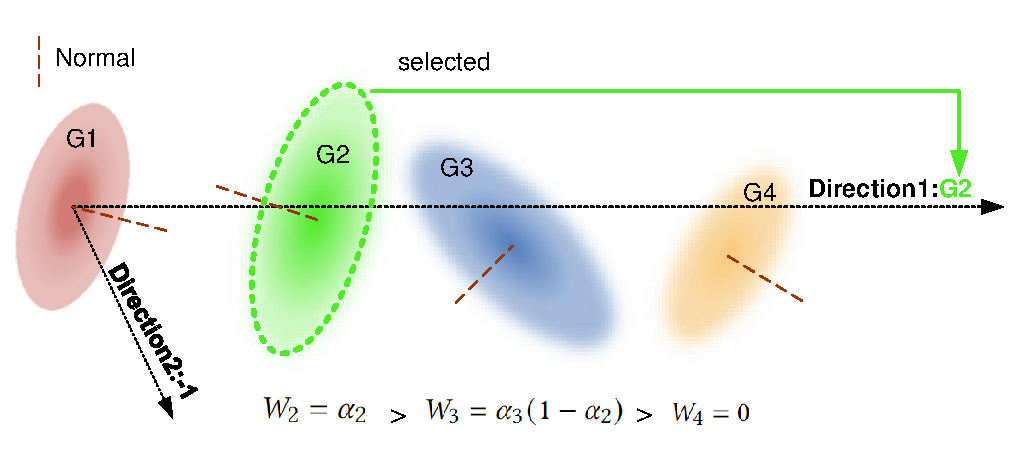
\includegraphics[width=\linewidth]{figures/raytracing.pdf}
\centering
 \vspace{-1cm}
\caption{3D Gaussian raytracing. Ray from $G_1$ at direction 1 hits 3 Gaussian splats $G_2$, $G_3$ and $G4$, we compute the weight for each Gaussian splat by equation \ref{weight} 
and select the Gaussian splat with the biggest weight ($G_2$).}

\label{raytracing}
 \vspace{-0.5cm}
\end{figure}
which is defined on sphere $\omega_i$ since $v$ is given.
According to equation \ref{prt sh}, we can simply precompute $T(x,\omega_i)$ into a transfer vector $\Vec{T}$. However, the previously mentioned approach is not applicable for computing self-transfer. This is due to the inconsistency in the $\omega_o$ for interreflection, leading to exponentially increasing computational complexity. 
By assuming that all indirect illumination originates from diffuse surfaces, we can streamline complicated matrix calculations into vector calculations. Additionally, we precompute the diffuse radiance transfer:
\begin{align}
    T_{diffuse}(x,\omega_i)=f_d(\omega_i \cdot n)V(\omega_i,x)
\end{align}
into $\Vec{T}_{diffuse}$. In sec \ref{4.4}, we precompute the index of other Gaussian splats $x'$ that exert the greatest contribution on the current Gaussian splat along direction $d_i$. Therefore, we can quickly query its corresponding diffuse radiance transfer $\Vec{T}_{diffuse}^{d_i}$. According to equation \ref{recu2}, one-bounce self-transfer can be written as:
\begin{align}
    T^{1}=f(d_i,v)(d_i \cdot n)\int_{\Omega}{T}_{diffuse}^{d_i}(\omega_i^{1},-d_i)d\omega_i^{1}
\end{align}
and
\begin{align}
   {T}_{diffuse}^{d_i}(\omega_i^{1})=\sum_{j=1}^{n^2}t_jY_j(\omega_i^{1})=\Vec{T}_{diffuse}^{d_i} \cdot \Vec{Y(\omega_i^{1})}
\end{align}
then:
\begin{align}
   T^{1}=\sum_{d_i}f(d_i,v)(d_i \cdot n)\Vec{T}_{diffuse}^{d_i} \cdot \Vec{Y(\omega_i^{1})}
\end{align}
and one-bounce diffuse self-transfer can be written as:
\begin{align}
   T_{diffuse}^{1}=\sum_{d_i}\frac{\rho}{\pi}(d_i \cdot n)\Vec{T}_{diffuse}^{d_i} \cdot \Vec{Y(\omega_i^{1})}
\end{align}

Recursively, we can compute n-bounce self-transfer.
\begin{align}
   T^{n}=\sum_{d_i}f(d_i,v)(d_i \cdot n)\Vec{T}_{diffuse}^{d_i,n-1} \cdot \Vec{Y(\omega_i^{n})} \label{self transfer}
\end{align}
Finally, the total self-transfer vector is:
\begin{align}
   \Vec{T}=\sum_{j=1}^{n}\Vec{T}^{j}
\end{align}
Although our method may not address specialized light paths (such as SDS path), it can efficiently compute simple specular interreflections (such as SD path) that \cite{liang2023gsir,gao2023relightable,shi2023gir} can't since current Gaussian splat is not assumed to be diffuse.
% \begin{table*}[htbp]
%   \centering
%       \caption{Quantatitive Comparison on TensoIR Synthetic dataset. Our method outperforms both previous offline and real-time methods on Novel view synthesis. Our relighting results rank first in all real-time methods and second in all methods, only behind TensoIR. Importantly, the average training time of our GS-IR is accelerated by a factor of 25x, and the average training time is accelerated by a factor of 10000x compared to TensoIR, making its performance acceptable and further demonstrating the effectiveness of our approach. For fairness, all methods are implemented by Python. Best \textbf{Real-Time} results are marked in pink, the second best are marked in orange. }
%     \resizebox{1.0\linewidth}{!}{
%     % \footnotesize
%     \scriptsize
%     \begin{tabular}{cc|ccc|ccc|cc}
%     \hline
%     \multirow{2}{*}{Category}& Method & \multicolumn{3}{c}{Novel View Synthesis} & \multicolumn{3}{c|}{Relighting} & \multirow{2}[1]{*}{ Render time} & \multirow{2}[1]{*}{ Train time} \\
%     \cline{2-8}
%     &Metircs & PSNR & SSIM& LPIPS & PSNR & SSIM& LPIPS &       &  \\
%     \hline
%     \multirow{3}{*}{Offline}&NeRFactor & 24.740 & 0.916 & 0.114  & 23.606  & 0.908  & 0.122  &      >100s  & >100h\\
%     &InvRender & 25.879 & 0.928 & 0.088  & 22.754  & 0.892  & 0.104  &   63.49s    & 15h \\
%     &TensoIR & 34.540 & 0.976 & 0.039  & \cellcolor {pink!80!orange}29.127  & \cellcolor {pink!80!orange}0.955  & \cellcolor {pink!80!orange}0.065  &>100s&  5h  \\
%     \hline
%     \multirow{4}{*}{RealTime}&NVDiffrec & 28.617 & 0.958 & \cellcolor {white!20}0.051  & 20.149  & 0.877  & \cellcolor {orange!25}0.083  & \cellcolor {pink!80!orange}0.005s & <1h \\
%     &Gsir  & \cellcolor {white!20}35.739 &\cellcolor {white!20} 0.975 & \cellcolor {orange!25}0.035  & \cellcolor {white!20}25.308  &\cellcolor {white!20} 0.884  & 0.096  &  - & <1h \\
%     &Relightable &\cellcolor {orange!25}39.204&\cellcolor {orange!25}0.984&0.059 & \cellcolor {orange!25} 27.017  &\cellcolor {orange!25} 0.893  & \cellcolor {orange!25}0.083  &  \cellcolor {white!20}0.022s   &  <1h \\
    
%     &Ours  & \cellcolor {pink!80!orange} \textbf{41.985} & \cellcolor {pink!80!orange} \textbf{0.988} & \cellcolor {pink!80!orange} \textbf{0.022}  & \cellcolor {pink!80!orange} \textbf{27.760}  &\cellcolor {pink!80!orange} \textbf{0.903}  & \cellcolor {pink!80!orange} \textbf{0.074}  &  \cellcolor {orange!25}0.013s   & <1h \\
%     \hline
    
%     \end{tabular}%
%     }

%   \label{tap_main}%
% \end{table*}%

% \begin{table*}[htbp]
%   \centering
%       \caption{Quantatitive Comparison on TensoIR Synthetic dataset. Our method outperforms both previous offline and real-time methods on Novel view synthesis. Our relighting results rank first in all real-time methods and second in all methods, only behind TensoIR. Importantly, the average training time of our PRTGS is accelerated by a factor of 25x, and the average training time is accelerated by a factor of 10000x compared to TensoIR, making its performance acceptable and further demonstrating the effectiveness of our approach. The best results are marked in red, the second best are marked in blue. }
%        \vspace{-0.3cm}
%     \resizebox{1.0\linewidth}{!}{
%     % \footnotesize
%     \scriptsize
    
%     \begin{tabular}{c|c|ccc|ccc|c|c}
%     \hline
%     \multirow{2}{*}{Category}& \multirow{2}{*}{Method} & \multicolumn{3}{c|}{Novel View Synthesis} & \multicolumn{3}{c|}{Relighting} & \multirow{2}[1]{*}{ Render time} & \multirow{2}[1]{*}{ Train time} \\
%     \cline{3-8}
%     & & PSNR$\tiny$$\uparrow$
%  & SSIM$\tiny$$\uparrow$& LPIPS$\tiny$$\downarrow$ & PSNR$\tiny$$\uparrow$ & SSIM$\tiny$$\uparrow$& LPIPS$\tiny$$\downarrow$ &       &  \\
%     \hline
%     \multirow{3}{*}{Offline}&NeRFactor & 24.740 & 0.916 & 0.114  & 23.606  & 0.902  & 0.122  &      >100s  & 4 days\\
%     &InvRender & 25.879 & 0.928 & 0.088  & 22.754  & 0.892  & 0.104  &   63.49s    & 15hours \\
%     &TensoIR& 34.540 & 0.976 & 0.039  & \textbf{\textcolor{red}{29.127}}  & \textbf{\textcolor{red}{0.955}}  & \textbf{\textcolor{red}{0.065}}  &>100s&  5 hours  \\
%     \hline
%     \multirow{4}{*}{RealTime}&NVDiffrec & 28.617 & 0.958 & \cellcolor {white!20}0.051  & 20.149  & 0.877  & {0.083}  & \textbf{\textcolor{red}{0.005s}} & 1 hour \\
%     &Gsir  & \cellcolor {white!20}35.739 &\cellcolor {white!20} 0.975 & \textbf{\textcolor{blue}{0.035}}  & \cellcolor {white!20}25.308  &\cellcolor {white!20} 0.884  & 0.096  &  - & minutes \\
%     &Relightable &\textbf{\textcolor{blue}{39.204}}&\textbf{\textcolor{blue}{0.984}}&0.059 & 27.017  &0.893  & 0.083  &  \cellcolor {white!20}0.022s   &  30 minutes \\
    
%     &Ours  & \textbf{\textcolor{red}{41.985}} & \textbf{\textcolor{red}{0.988}} & \textbf{\textcolor{red}{0.022}}  & \textbf{\textcolor{blue}{27.76}}  &\textbf{\textcolor{blue}{0.903}}  &  \textbf{\textcolor{blue}{0.074}}  &  \textbf{\textcolor{blue}{0.013s}}   & 35 minutes \\
%     \hline
%      \vspace{-0.3cm}
%     \end{tabular}%
% }

%   \label{tap_main}%
% \end{table*}%
\begin{table*}[htbp]
\centering
\caption{Quantitative Comparison on TensoIR Synthetic Dataset. Our method outperforms both previous offline and real-time methods on Novel View Synthesis. Our relighting results rank first in all real-time methods and second in all methods, only behind TensoIR. Importantly, the average training time of our PRTGS is accelerated by a factor of 25$\times$, and the average training time is accelerated by a factor of 10000$\times$ compared to TensoIR, making its performance acceptable and further demonstrating the effectiveness of our approach. The best results are marked in red, the second best are marked in blue.}
\vspace{-0.3cm}
\resizebox{1.0\linewidth}{!}{
\begin{tabular}{c|c|ccc|ccc|c|c}
\hline
\multirow{2}{*}{Category} & \multirow{2}{*}{Method} & \multicolumn{3}{c|}{Novel View Synthesis} & \multicolumn{3}{c|}{Relighting} & \multirow{2}{*}{Render Time} & \multirow{2}{*}{Train Time} \\
\cline{3-8}
& & PSNR$$\tiny$$$\uparrow$ & SSIM$\tiny$$\uparrow$ & LPIPS$\tiny$$\downarrow$ & PSNR$\tiny$$\uparrow$ & SSIM$\tiny$$\uparrow$ & LPIPS$\tiny$$\downarrow$ & & \\
\hline
\multirow{3}{*}{Offline} & NeRFactor & 24.740 & 0.916 & 0.114 & 23.606 & 0.902 & 0.122 & >100s & 4 days \\
& InvRender & 25.879 & 0.928 & 0.088 & 22.754 & 0.892 & 0.104 & 63.49s & 15 hours \\
& TensoIR & 34.540 & 0.976 & 0.039 & \textbf{\textcolor{red}{29.127}} & \textbf{\textcolor{red}{0.955}} & \textbf{\textcolor{red}{0.065}} & >100s & 5 hours \\
\hline
\multirow{4}{*}{RealTime} & NVDiffrec & 28.617 & 0.958 & 0.051 & 20.149 & 0.877 & 0.083 &0.005s & 1 hour \\
& Gsir & 35.739 & 0.975 & \textbf{\textcolor{blue}{0.035}} & 25.308 & 0.884 & 0.096 & - & minutes \\
& Relightable & \textbf{\textcolor{blue}{39.204}} & \textbf{\textcolor{blue}{0.984}} & 0.037 & 26.451 & 0.923 & 0.078 & 0.01s & minutes \\
& PRTGS (Ours) & \textbf{\textcolor{red}{41.985}} & \textbf{\textcolor{red}{0.988}} &  \textbf{\textcolor{red}{0.022}} &  \textbf{\textcolor{blue}{28.964}} &  \textbf{\textcolor{blue}{0.952}} &  \textbf{\textcolor{blue}{0.068}} & 0.015s &minutes \\
\hline
\end{tabular}
}
\label{tab_main}
\end{table*}
% \begin{table*}[htbp]
%   \centering
%       \caption{Quantatitive Comparison on TensoIR Synthetic dataset. Our method outperforms both previous offline and real-time methods on Novel view synthesis. Our relighting results rank first in all real-time methods and second in all methods, only behind TensoIR. Importantly, the average training time of our GS-IR is accelerated by a factor of 25x, and the average training time is accelerated by a factor of 10000x compared to TensoIR, making its performance acceptable and further demonstrating the effectiveness of our approach. For fairness, all methods are implemented by Python. Best \textbf{Real-Time} results are marked in pink, the second best are marked in orange. }
%     \resizebox{1.0\linewidth}{!}{
%     % \footnotesize
%     \scriptsize
%     \begin{tabular}{cc|ccc|ccc|cc}
%     \hline
%     \multirow{2}{*}{Category}& Method & \multicolumn{3}{c}{Novel View Synthesis} & \multicolumn{3}{c|}{Relighting} & \multirow{2}[1]{*}{ Render time} & \multirow{2}[1]{*}{ Train time} \\
%     \cline{2-8}
%     &Metircs & PSNR & SSIM& LPIPS & PSNR & SSIM& LPIPS &       &  \\
%     \hline
%     \multirow{3}{*}{Offline}&NeRFactor & 24.740 & 0.916 & 0.114  & 23.606  & 0.908  & 0.122  &      >100s  & >100h\\
%     &InvRender & 25.879 & 0.928 & 0.088  & 22.754  & 0.892  & 0.104  &   63.49s    & 15h \\
%     &TensoIR & 34.540 & 0.976 & 0.039  & \cellcolor {pink!80!orange}29.127  & \cellcolor {pink!80!orange}0.955  & \cellcolor {pink!80!orange}0.065  &>100s&  5h  \\
%     \hline
%     \multirow{4}{*}{RealTime}&NVDiffrec & 28.617 & 0.958 & \cellcolor {white!20}0.051  & 20.149  & 0.877  & \cellcolor {orange!25}0.083  & \cellcolor {pink!80!orange}0.005s & <1h \\
%     &Gsir  & \cellcolor {white!20}35.739 &\cellcolor {white!20} 0.975 & \cellcolor {orange!25}0.035  & \cellcolor {white!20}25.308  &\cellcolor {white!20} 0.884  & 0.096  &  - & <1h \\
%     &Relightable &\cellcolor {orange!25}39.204&\cellcolor {orange!25}0.984&0.059 & \cellcolor {orange!25} 27.017  &\cellcolor {orange!25} 0.893  & \cellcolor {orange!25}0.083  &  \cellcolor {white!20}0.022s   &  <1h \\
    
%     &Ours  & \cellcolor {pink!80!orange} \textbf{41.985} & \cellcolor {pink!80!orange} \textbf{0.988} & \cellcolor {pink!80!orange} \textbf{0.022}  & \cellcolor {pink!80!orange} \textbf{27.760}  &\cellcolor {pink!80!orange} \textbf{0.903}  & \cellcolor {pink!80!orange} \textbf{0.074}  &  \cellcolor {orange!25}0.013s   & <1h \\
%     \hline
    
%     \end{tabular}%
%     }

%   \label{tap_main}%
% \end{table*}%
% \begin{table*}[htbp]
%   \centering
%     \resizebox{1.0\linewidth}{!}{
%     % \footnotesize
%     \scriptsize
%     \begin{tabular}{c|ccc|ccc|cc}
%     \hline
%     Method & \multicolumn{3}{c}{Novel View Synthesis} & \multicolumn{3}{c|}{Relighting} & \multirow{2}[1]{*}{AVG Train time} & \multirow{2}[1]{*}{AVG Render time} \\
%     \cline{0-6}
%     Metircs & PSNR & SSIM& LPIPS & PSNR & SSIM& LPIPS &       &  \\
%     \hline
%     NeRFactor & 24.740 & 0.916 & 0.114  & 23.606  & \cellcolor {orange!25}0.908  & 0.122  &    >100h   &  >100s\\
%     InvRender & 25.879 & 0.928 & 0.088  & 22.754  & 0.892  & 0.104  &   15h    &  63.49s \\
%     NVDiffrec & 28.617 & 0.958 & 0.051  & 20.149  & 0.877  & \cellcolor {yellow!20}0.083  &  \cellcolor {pink!80!orange}<1h     & \cellcolor {pink!80!orange}0.005s \\
%     Gsir  & \cellcolor {yellow!20}35.739 & 0.975 & \cellcolor {yellow!20}0.035  & 25.308  & 0.884  & 0.096  &    \cellcolor {pink!80!orange}<1h   &  -\\
%     Relightable &\cellcolor {orange!25}39.204&\cellcolor {orange!25}0.984&0.059 & \cellcolor {yellow!20} 27.017  & 0.893  & \cellcolor {yellow!20}0.083  &    \cellcolor {pink!80!orange}<1h   & \cellcolor {yellow!20}0.022s \\
%     TensoIR & 34.540 &\cellcolor {yellow!20} 0.976 & \cellcolor {orange!25}0.039  & \cellcolor {pink!80!orange} \textbf{29.127}  & \cellcolor {pink!80!orange} \textbf{0.955}  & \cellcolor {pink!80!orange} \textbf{0.065}  &    5h   & >100s \\
%     Ours  & \cellcolor {pink!80!orange} \textbf{41.985} & \cellcolor {pink!80!orange} \textbf{0.988} & \cellcolor {pink!80!orange} \textbf{0.022}  & \cellcolor {orange!25}27.760  &\cellcolor {yellow!20} 0.903  & \cellcolor {orange!25}0.074  &   \cellcolor {pink!80!orange}<1h    & \cellcolor {orange!25}0.013s \\
%     \hline
%     \end{tabular}%
%     }
%     \caption{Quantatitive Comparison on TensoIR Synthetic dataset. Our method outperforms both previous offline and real-time methods on Novel view synthesis. Our relighting results ranks first in all real-time methods and second in all method, only behind TensoIR. Importantly, the average training time of our GS-IR is accelerated by a factor of 25x and average training time is accelerated by a factor of 10000x comapred to TensoIR, making its performance acceptable and further demonstrating the effectiveness of our approach. For fairness, all methods are implemented by Python. }
%   \label{tap_main}%
% \end{table*}%

\hupar{Transfer Matrix for unknown direction} During relighting and other test tasks, we can precompute the transfer matrix for glossy cases since BRDF and other properties are certain. Given:
\begin{align}
    T(x,\omega_i,\omega_o)=(f_d+f_s(\omega_i,\omega_o))(\omega_i \cdot n)V(\omega_i,x)
\end{align}
According to equation \ref{sh_jifen}, we have:
\begin{align}
    t_i(\omega_o)=\int T(\omega_o,\omega_i)Y_i(\omega_i)d\omega_i
\end{align}  
$t_i(\omega_o)$ is defined on the sphere $\omega_o$, so it can be represented as another set of basis functions:
\begin{align}
    t_i(\omega_o)=\sum_{j=1}^{n^2}t'_{ij}Y_j(\omega_o)
\end{align}
and $T(\omega_o,\omega_i)$ can be represented as:
\begin{align}
    T(\omega_o,\omega_i)=\sum_{i=1}^{m^2}\sum_{j=1}^{n^2}t'_{ij}Y_j(\omega_o)Y_i(\omega_i)
\end{align}
where:
\begin{align}
    t'_{ij}=\sum_{l=1}^{q}\sum_{k=1}^{p}Y_i(\omega_i^l)T(\omega_i^l,\omega_o^l)Y_j(\omega_o^k)
    \label{glossy prt}
\end{align}
Here we sample $\omega_i$ m times and $\omega_o$ p times. Then equation \ref{prt} can be written as:
\begin{align}
    L_o(x)=\sum_{i=0}^{m^2}\sum_{j=0}^{n^2}l_it'_{ij}=\Vec{L} \cdot T_{m \times n}
\end{align}
Like \ref{self transfer}, we can precompute self-transfer 
% \begin{align}
%     t'_{ij}^{n} &= \sum_{k} \alpha \left( f(d_i,v)(d_i \cdot n) \right) \left( t'_{kj} \right){1}_{d_i}^{n-1} \cdot Y_k(-d_i) Y_j(d_i)
% \end{align}


However, we still opt for diffuse self-transfer in most cases due to its faster computation.

\begin{figure*}[htbp]
 \vspace{-0.3cm}
\centering
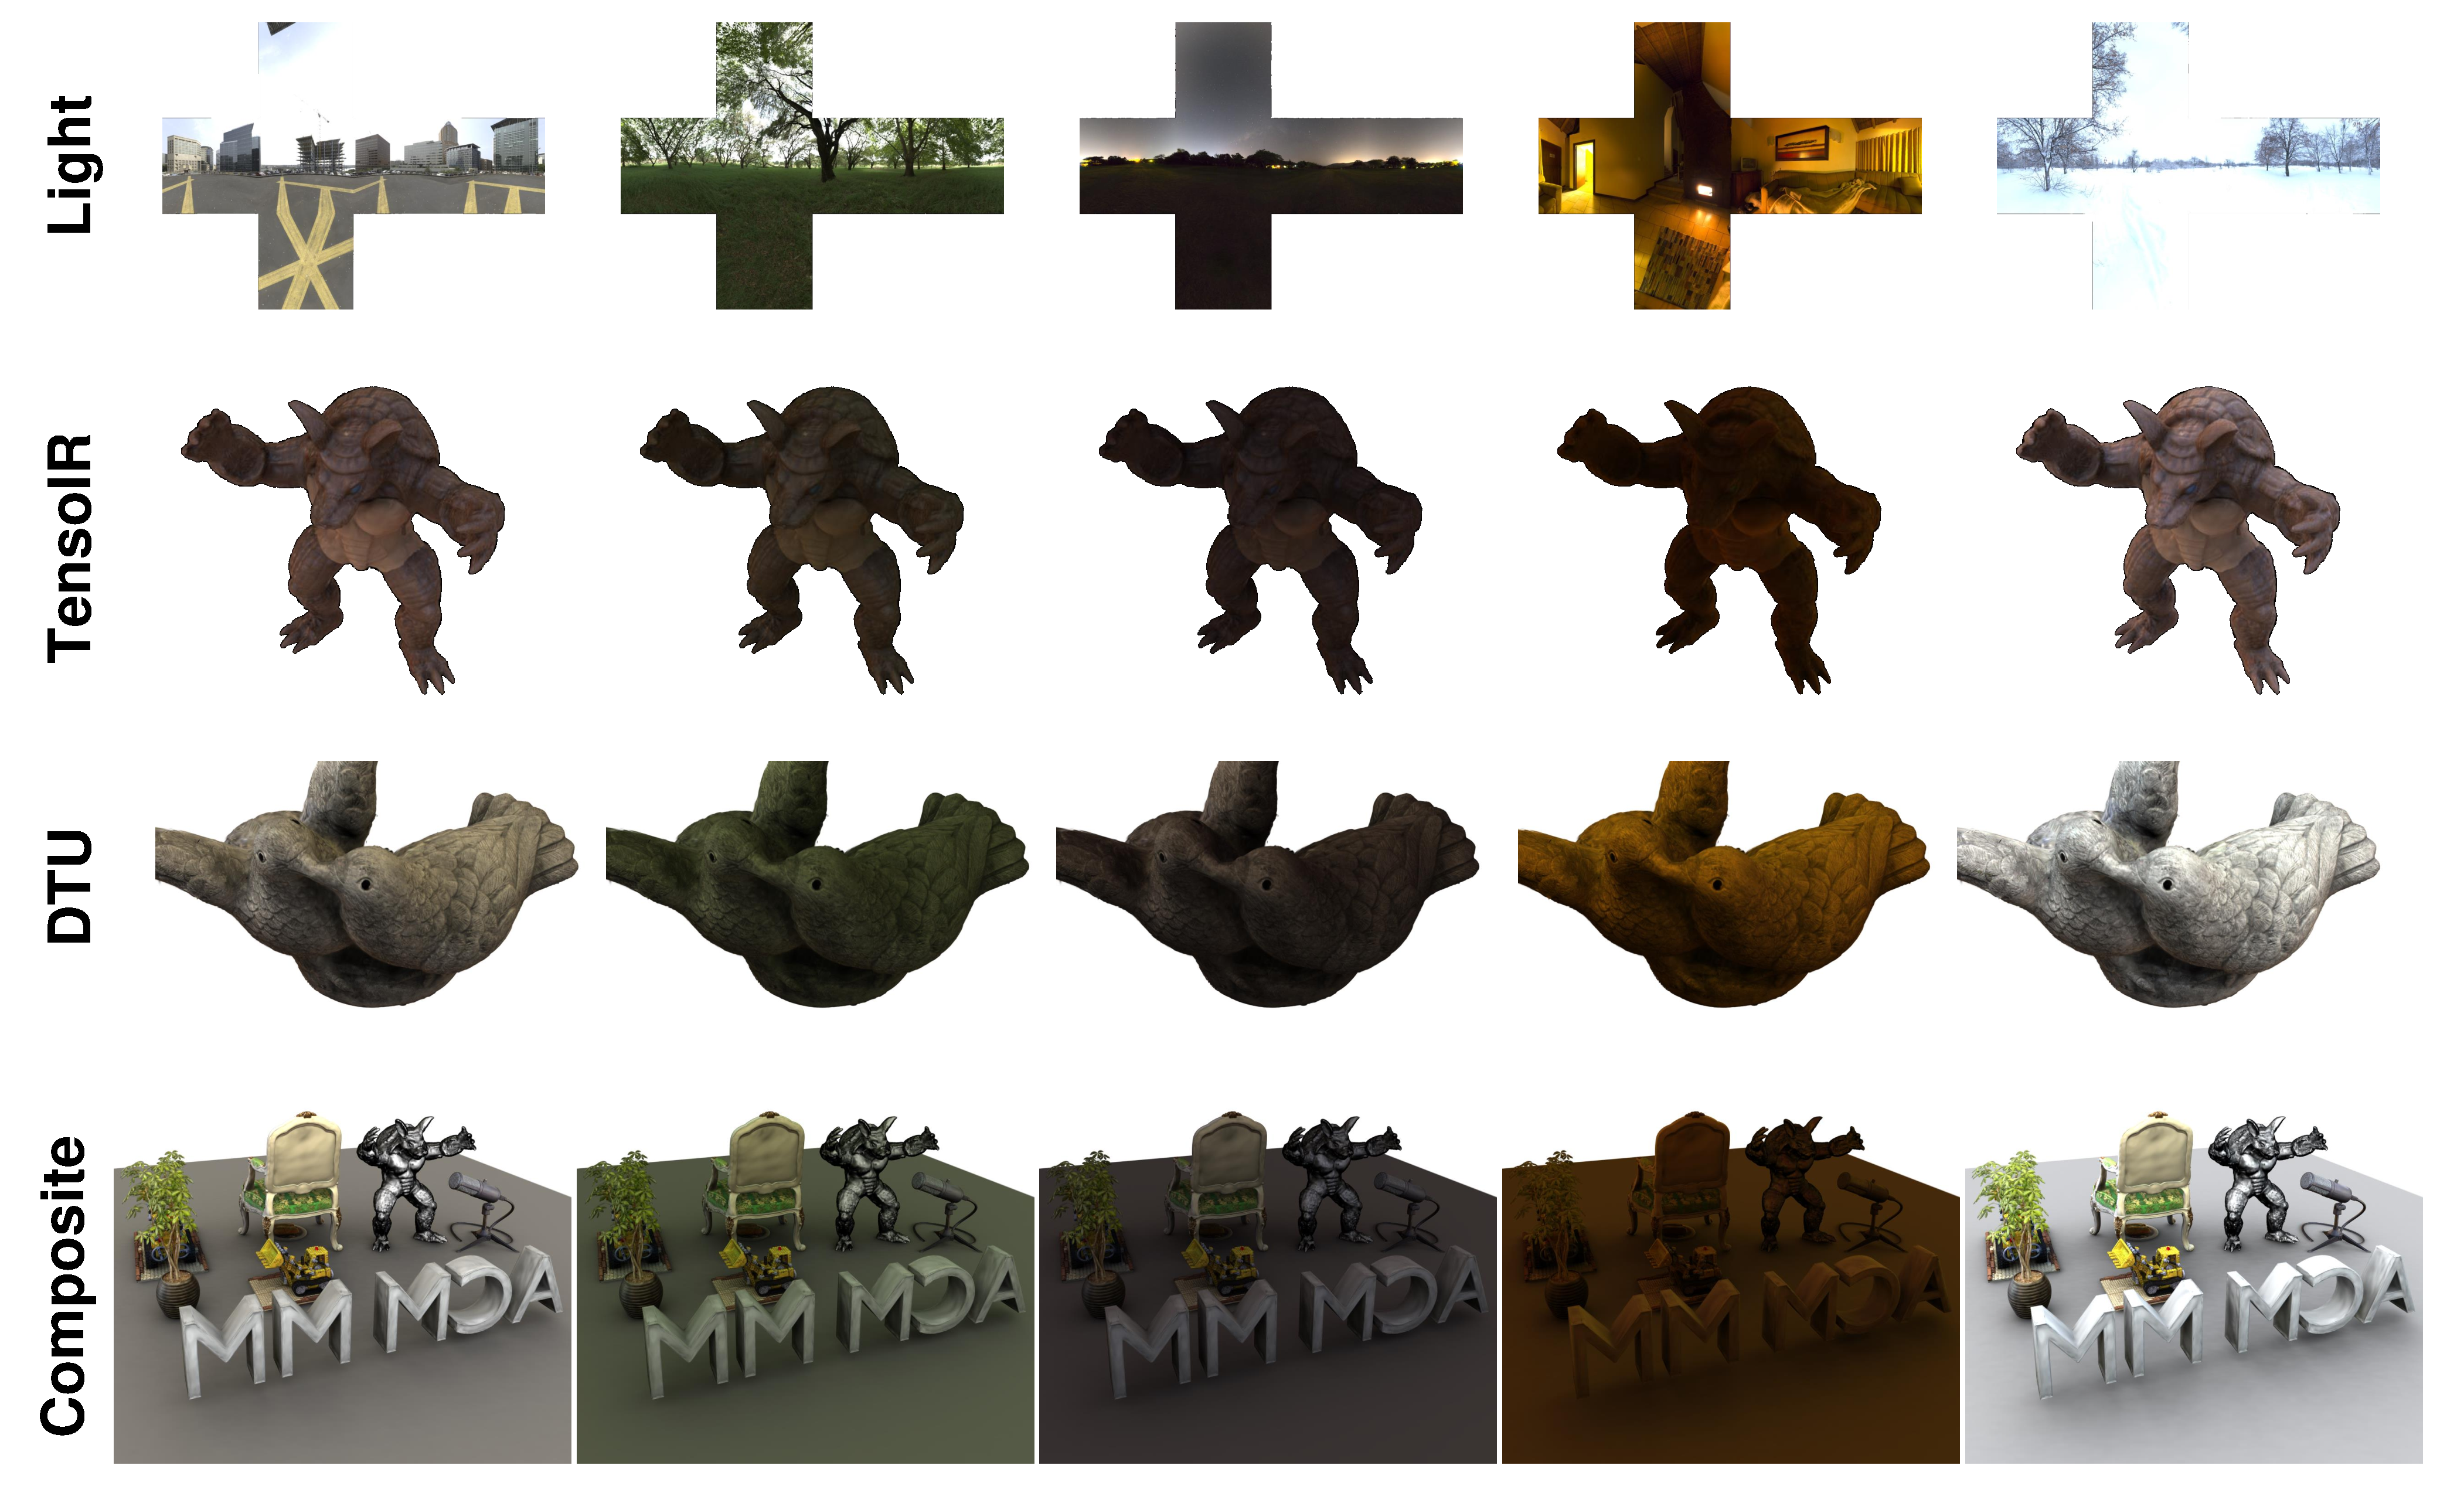
\includegraphics[width=\linewidth]{figures/main.pdf}
 \vspace{-0.3cm}
\caption{High-quality relighting results achieved by our proposed method on TensoIR dataset \cite{jin2023tensoir}, DTU dataset \cite{jensen2014large} and a composite scene created by us.}\label{main}
 \vspace{-0.3cm}
\end{figure*}